\chapter{Simulations}
\section{Plasma simulations}
%The accuracy by which modern plasma simulation codes are able to model plasma behaviour has made them a crucial part of current plasma physics research. 
Numerical simulations are a crucial part of plasma physics research. The accuracy by which modern plasma simulation codes are able to model plasma behaviour allows us to better understand and improve the functioning of our current experiments, as well as to explore and develop new novel ideas without the technological and financial limitations of real-world experiments. As a result, simulation studies play an increasingly more decisive role in guiding and accelerating current plasma wakefield research. \\
\indent Given that a plasma is, to a good approximation, nothing more than electrons and ions interacting electromagnetically, the response of such a plasma to the propagation of an electron beam or laser pulse could in theory be simulated by solving Maxwell's equations and calculating the Lorentz force law for each electron and ion in the plasma. This approach is however computationally intractable due to vast number of particles present in the simulations we need to perform. We circumvent this computational road block by making use of so-called Particle-In-Cell (PIC) codes. In this chapter we outline the general PIC approach and introduce the plasma physics PIC code EPOCH, which is used throughout this project. We further detail the modifications necessary to allow the hybrid beam dump scheme to be simulated with EPOCH. 



%Simulations because: Cheaper than experiments, more readily available to anyone, simulations allow us to study, understand and exploit these phenomena without the need to repeatedly perform expensive and intricate experiments...Furthermore, by having a simulated rather than physical experiment, one may avoid the uncertainties and noise present in the real world and may therefore investigate and even discover physical phenomena that are too sensitive to be detected in noisy data samples. 

%To take advantage of simulations it is however crucial to know the accuracy by which the simulations model the physical situation and to understand the limitations that this imposes. For instance, as will be shown in section XXX, failing to model the experiment with high enough resolution can lead to phenomena emerging from purely numerical features in the simulations. One must therefore be confident that the results seen in simulations accurately represent the physics at hand, either by comparing the simulations to experimental data or theoretical calculations if available. The non-linear nature of the high-energy plasma wakefield phenomena that we wish to model in this project do not lend themselves easily to analytical treatments. To investigate these phenomena and provide useful results for future experiments we will make extensive use of simulations in this project.\\ 



%In this chapter we introduce the plasma physics PIC code EPOCH, which is used throughout this project, and detail the modifications necessary to allow the hybrid beam dump scheme to be simulated. 

%The behaviour of these macro particles is then calculated and used as a representation of the response of the actual plasma.  where each macroscopic particle carries the total charge and mass of the microscopic particles it represents. 



\section{Particle-in-Cell Codes}
\label{sec:Particle-in-Cell Codes}
The key feature of all PIC codes is to represent a large ensemble of microscopic particles by a smaller ensamble of macroscopic pseudo-particles on a discrete spatial grid \cite{Pukhov2015}. Each of these macroparticles carries the total charge and mass of the collection of electrons or ions that it represents and, importantly, are not point particles but finite regions of space, 'cells', that move as one. The interactions and dynamical behaviour of these macroparticles is then used as a representation of the actual plasma response. This significantly reduces the computational cost. A further simplifying feature of PIC codes is that the EM fields are only calculated on discrete points on a so-called Yee grid whilst the macroparticles move continuously through this grid, ensuring that accurate dynamical behaviour is maintained \cite{Lawrence-Douglas2013}. Hence, once a distribution of moving charged particles has been introduced into this grid the EM fields can be computed by solving Maxwell's equations in discretized time, which in turn govern the subsequent motion on the particles. However, the fact that the discrete space of fields is disjoint from the continuous field of particles means that we need an approach to translate between them. We outline the general method to do this in figure \ref{PIC_loop}, which involves an iterative loop of so-called particle push and field solver algorithms. We start by considering a known spacial distribution of particles and their associated velocities, $\left(\boldsymbol{r}_{n},\boldsymbol{v}_{n}\right)$, at a time $t_n$. In order to compute the the induced EM fields at discrete grid points the charged macroparticles are weighted onto several of the nearest grid points, thus resulting in each grid point having an associated charged distribution and current, $\left(\rho_{n},\boldsymbol{J}_{n}\right)$. The corresponding EM fields, which we label by $n+1$ since these will act to move our particles, are found through Maxwell's equation via a \textit{field solver} algorithm. This is necessitated by the fact that the EM fields at n+1, $\left(\boldsymbol{E}_{n+1},\boldsymbol{B}_{n+1}\right)$, are not only sourced by $\rho_{n}$ and $\boldsymbol{J}_{n}$ but also by the variation of the fields, $\Delta\vec{B}$ and $\Delta\vec{E}$, between $n$ and $n+1$ through Ampere's and Faraday's laws. Hence the fields can not be computed at the same time since, for instance, $\vec{B}_{n+1 }$ is in part induced by $\Delta\vec{E}=\vec{E}_{n+1}-\vec{E}_n$, where $\vec{E}_{n+1}$ is in turn induced by $\Delta\vec{B}=\vec{B}_{n+1}-\vec{B}_n$. This issue is addressed by the \textit{leapfrog} method, whereby particle positions and velocities are calculate at alternating half-way intermediate steps $n+1/2$, but out of step by $\Delta t/2$. This means that we compute $\boldsymbol{r}_{n}$ and $\boldsymbol{v}_{n-1/2}$ simultaneously, followed by $\boldsymbol{r}_{n+1}$ and $\boldsymbol{v}_{n+1/2}$. Although not immediately obvious, this allows us to calculate the EM fields in the following chain: $\left(\vec{E}_n,\vec{B}_n\right) \to (\vec{E}_n,\vec{B}_{n+1/2}) \to (\vec{E}_{n+1},\vec{B}_{n+1/2})  \to  (\vec{E}_{n+1},\vec{B}_{n+1})$. It can further be shown that the truncation error per iteration scales as the square of the distance successive grid points \cite{Lawrence-Douglas2013}, and is thus a second-order numerical simulation scheme. Once these fields are known the first step of the loop is effectively done in reverse by weighting the fields off the grid and back onto each individual macroparticle. Then using a similar leapfrog method in a \textit{particle pusher} algorithm the Lorentz force law is used to push the particles to their new positions and velocities, thus completing the iteration step. 
%\begin{figure}
%\centering
%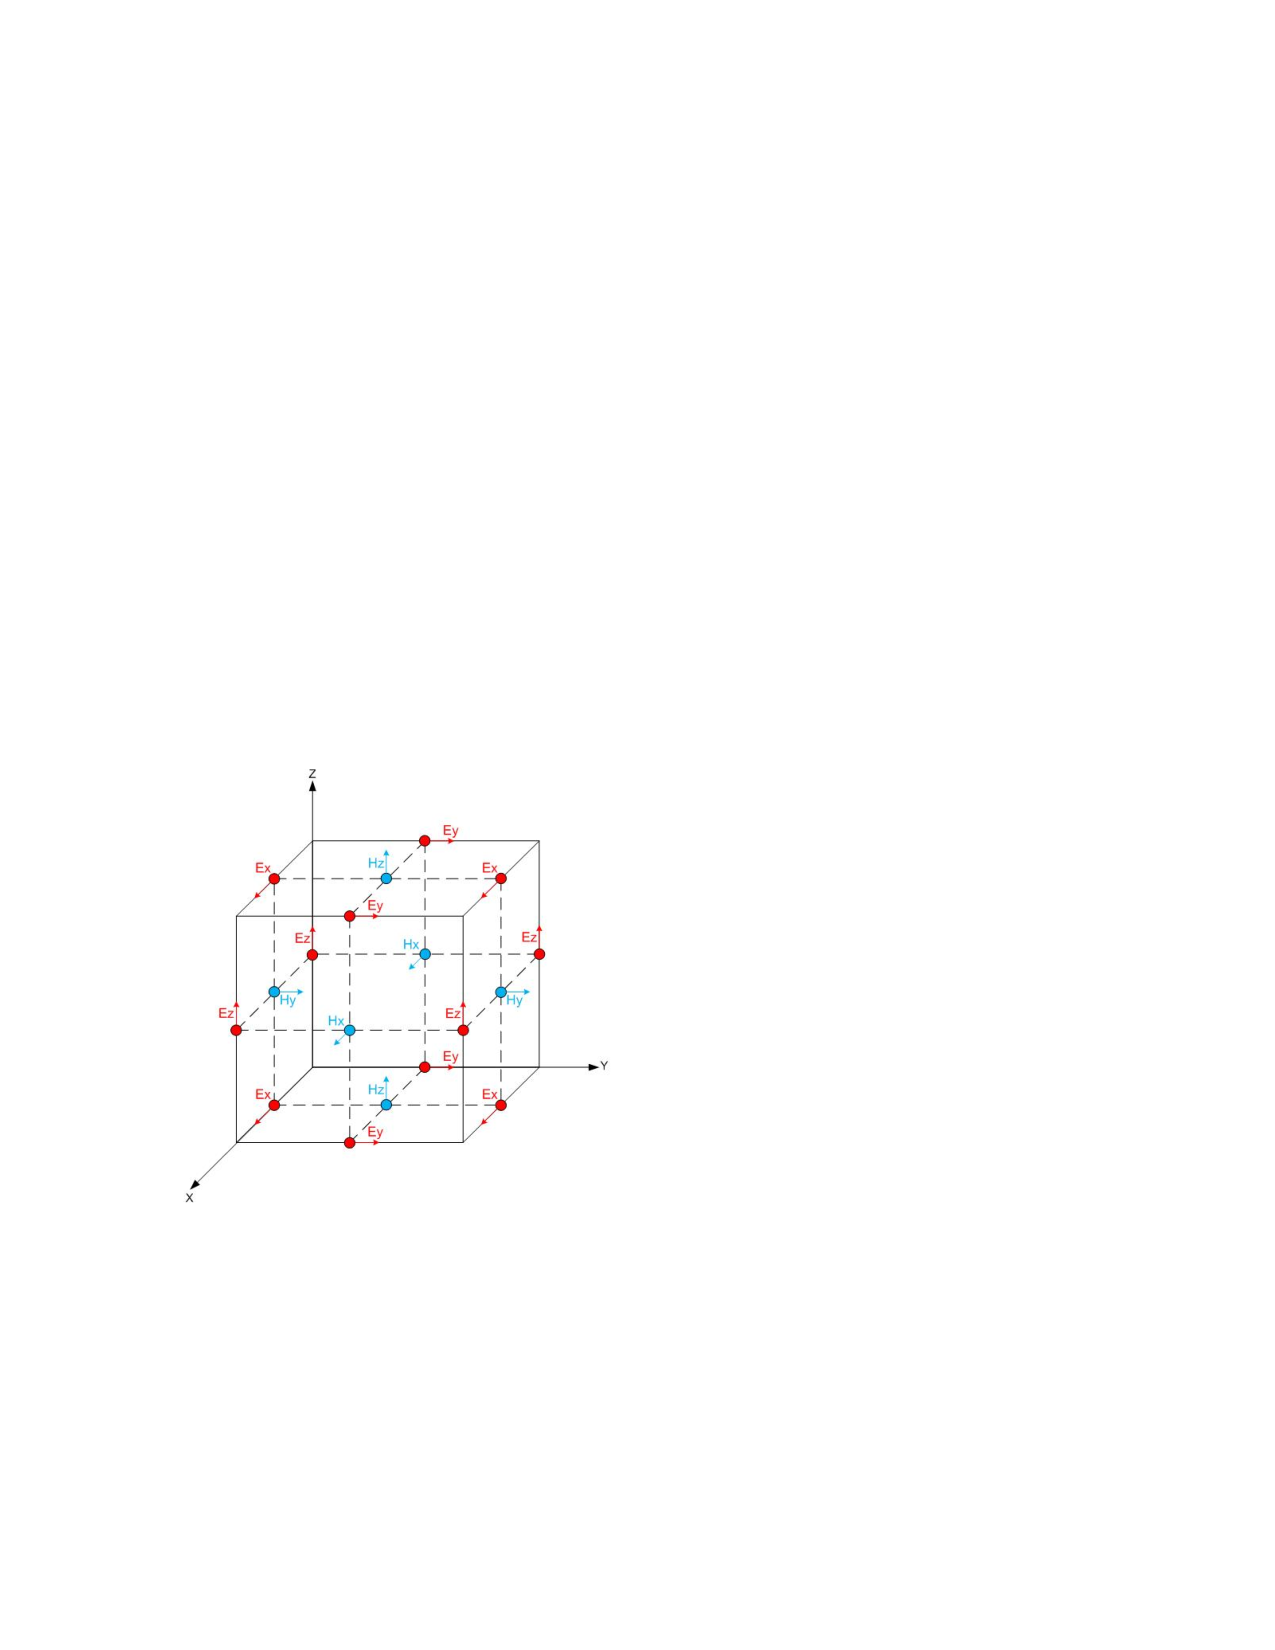
\includegraphics[width=0.5\textwidth]{YeeGrid.pdf}
%\caption{Flowchart showing the general operations conducted during one time iteration of the Particle-In-Cell simulation method. The colours indicate whether the EM fields and particle distributions are calculated at points on the discretized Yee grid (orange) or in the continuous space of particles (blue). The field update and particle push algorithms}
%\label{PIC_loop}
%\end{figure}
\begin{figure}
\centering
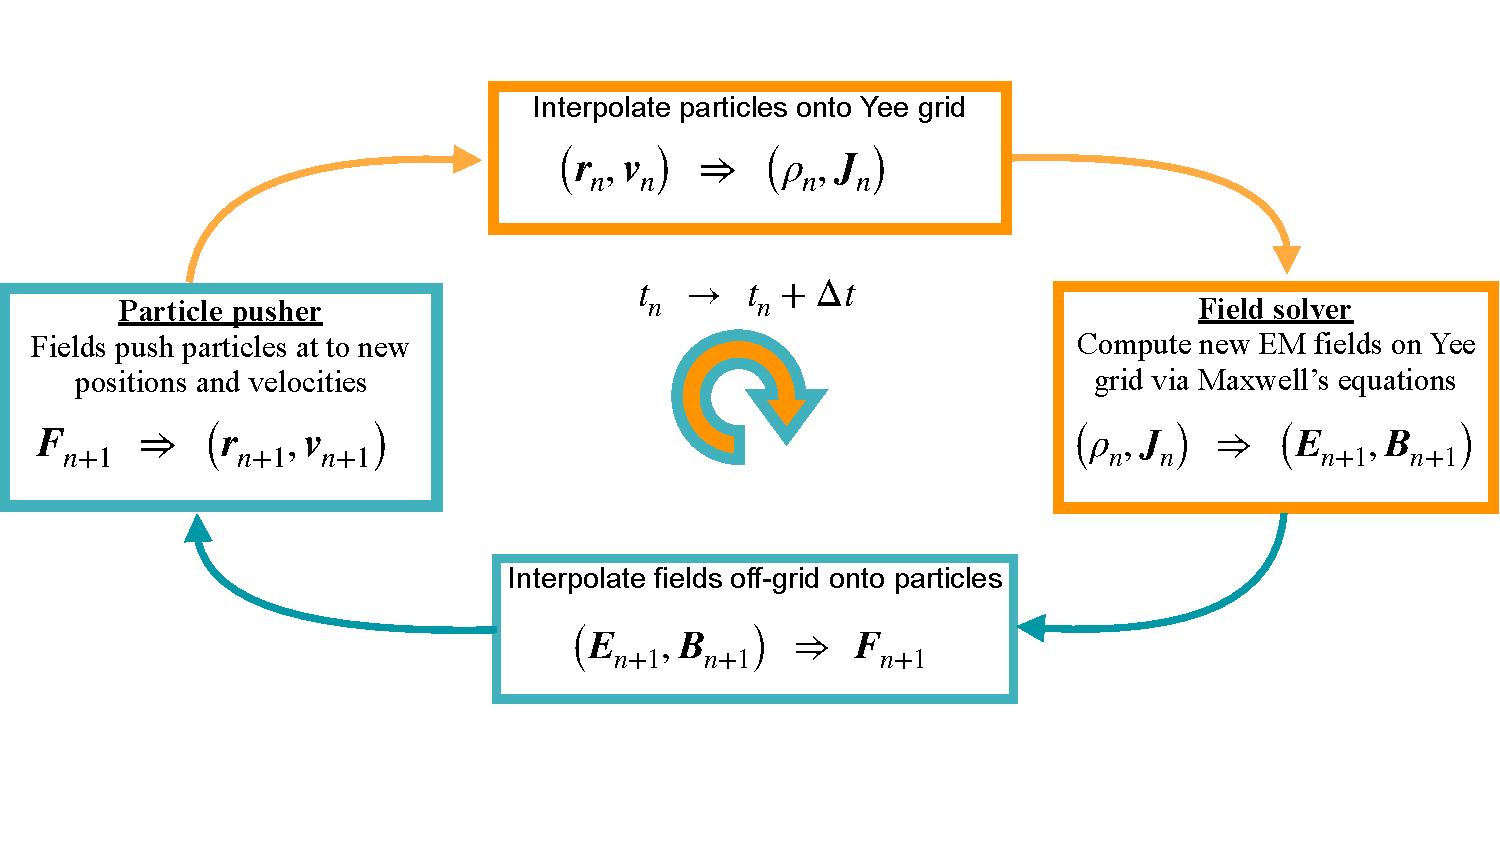
\includegraphics[width=\textwidth]{PIC_loop2.pdf}\vspace{-30pt}
\caption{\small{Flowchart showing the general operations conducted during one time iteration of the Particle-In-Cell simulation method. The colours indicate whether the EM fields and particle distributions are calculated at points on the discretized Yee grid (orange) or in the continuous space of particles (blue). The field update and particle push algorithms}}
\label{PIC_loop}
\end{figure}


\section{EPOCH}
%The simulations presented in this thesis are generated using the open-source plasma physics PIC simulation code \textsc{EPOCH},
The Extensible PIC Open Collaboration project (EPOCH) is an advance relativistic electromagnetic PIC code developed at the University of Warwick \cite{Bennett2015}. EPOCH is now maintained and developed through the Collaborative Computational Project in Plasma Physics (CCP-Plasma), from which access to the code is granted to non-profit research laboratories and Universities \cite{ChrisBRADYKeithBENNETTHolgerSCHMITZ}. 
%Simulations  using EPOCH simply require users to specify the parameters and initial conditions of the simulations without the need to interact with the underlying PIC code.
The underlying code is written in Fortran and allows for simulations to be run on multiple parallel processors via MPI; this enables time-consuming simulations to be run on remote computing clusters. The core PIC code in EPOCH is based upon the field solver and particle push algorithms of the Plasma Simulation Code (PSC) written by H. Ruhl \cite{Ruhl}. This follows closely the standard PIC scehme outline in section \ref{sec:Particle-in-Cell Codes}. The main difference being the use of a more precise leapfrog method and the inclusion of additional functionality to allow for more advanced features such as collisions, ionisation and quantum electrodynamic radiation to be simulated. Furthermore, EPOCH is highly user-friendly; setting up simulations simply requires users to specify the parameters and initial conditions of the simulations without the need to interact with the underlying PIC code. Likewise, analysing and visualising data from a simulations is made easier through file-compatibility with Python, Matlab, IDL and VisIt.
\subsection{Input deck}
Once EPOCH has been downloaded and compiled the  \textit{input deck} is essentially EPOCH's user interface. This is a text file in which users specify the details of a simulation to be passed onto EPOCH's core PIC algorithm. It is composed of blocks which each specify different features of the simulations. The full details of all available blocks can be found in the EPOCH user manual \cite{Bennett2015}. The control, species and laser blocks are of particular importance to this project and will be covered briefly.  In the \textit{control block} the grid resolution, iteration time-steps and further details of the PIC scheme are specified. When defining the resolution of the grid one has to make sure that the grid is sufficiently fine such that the smallest features of our physical system are resolved. This is to ensure that the simulation accurately models the physical system it is meant to represent, to the extent that missing small-scale phenomena might alter the large scale outcome of the simulation. For instance, for laser-plasma interactions the wavelength of the laser ($\sim 500$ nm) needs to be resolved by the grid spacing to ensure that the induced electron-oscillations are accurately modelled. A finer grid however requires more macroparticles to fully populate the grid, which inevitably extends the computational time.The grid is populated through \textit{species block} where each species of particle, such as plasma electrons, plasma ions and electron beam driver, has a separate block. In these blocks, the number of macroparticels is specified together with the spatial and kinetic distributions of the particles. This allows us to, for instance, define a 1 GeV spherical electron bunch propagating through plasma with uniform or varying density. The introduction of a laser in the simulation is handled by the \textit{laser block}, where parameters such as the laser intensity, pulse length and spot-size are defined. This differs from the species block in that the laser has to be attached to one edge of the simulation window and fired at $t=0$, whereas the electron bunch can be initialised at any position at $t=0$. \\
\indent This posses two immediate issues for simulating the hybrid scheme: we require the laser to appear in front of the electron bunch, see figure \ref{hybrid_outline}(iv), while the current approach seems to at best allow us to initialise both the laser and bunch on top of each other at the beginning of the simulation window; we require the laser to fire after the bunch deceleration has saturated, see figure \ref{hybrid_outline}(iii), which is significantly after $t=0$. The former of these issues was resolved by features in the input deck alone. Specially, it was found that the bunch could be initialised and held stationary for a given amount of time, such that a stationary bunch could be initialised ahead of the laser and subsequently released once the laser had propagated through and past then bunch. This approach however appeared to still affect the bunch, to the extent that high enough intensity lasers would pass through and disintegrate the stationary bunch. A work-around was found by setting the intensity of the laser to zero until it had passed the bunch, at which point the intensity was increased linearly to its maximum value. Although this solves both of the issues above, since the intensity could be kept zero until the bunch saturates, there are good reasons to seek a more efficient approach. The primary one being the computational cost of running these simulations. Indeed, even though we have been granted access to 24 Intel cores on the High-Performance Computing (HPC) cluster at the University of Manchester \cite{CSF}, many of the simulations we need to perform still require a few days up to to several weeks to finish. This would make the process of optimizing any parameters in the more intricate active beam dump very time-consuming, since the passive beam dump would have to be simulated again following each minor change to the laser parameters for instance. It is therefore advantageous to divide up the simulation into separate passive and active beam dump simulations, where the latter then requires us to initialise a pre-saturated electron bunch together with a laser pulse.
%This requires us to simulate a laser pulse propagating in front of a pre-saturated bunch.
Crucially, however, the distributions functions in the input deck can only be defined analytically. Since previous studies \cite{Wu2010, Bonatto2015, Hanahoe2017} have shown that both the spatial and kinetic distributions of the electron driver after passing through a passive beam dump are highly non-analytical it is imperative that this issue be addresses if the hybrid beam dump is to be accurately simulated. 

%specifically by addressing the latter of the issues above; 

%The control and species blocks together define the resolution of the simulation. When setting up the resolution of the grid one has to make sure that the grid is sufficiently fine such that the smallest features of our physical system are resolved. This is to ensure that the simulation accurately models the physical system it is meant to represent, to the extent that missing small scale phenomena might alter the large scale outcome of the simulation. A finer grid however requires more macroparticles to fully populate the grid, which inevitably extents the computational time. In addition the time step $\Delta t$ aneeds to be suitably decreased as well. This is because of the so-called Courant-Friedrichs-Lewy (CFL) condition.  Any simulation introduces uncertainties in the final outcome due to the finite resolution. We need to make sure that the uncertainties introduces during each iteration do not build up and grow unbounded. \\

\subsection{Non-analytical bunch initialisation}
The hybrid scheme approach that the endeavour to investigate in this project relies on us being able to simulate a laser pulse propagating in front of a pre-saturated bunch. 
This was achieved by first exporting the data of the saturated bunch from a a passive beam dump simulation. The Self-Describing-File (SDF) data format used by EPOCH, however, is not suitable for easy access and retrieval of particular sets of data. A work-around was found by using the data-visualisation software VisIt \cite{LANL2005} to read the files and export only the data related to the macroparticles of the electron bunch into a text file. In order to import this into a new simulation it was necessary to over-ride the electron bunch parameters in the input deck. Fortunately, EPOCH provides a file, \texttt{icmodule.f90}, which allows users to assigning custom values to each of the macroparticles that have been initialised in in the input deck. Hence, by initialising a standard spherical electron bunch in the input deck with the exact number of macroparticles that we exported from the passive simulation and reading in the exported data in the \texttt{icmodule.f90} file, we were able to loop over these particles and assign each one with a new charge, mass, position and velocity corresponding to a macroparticle in the exported data file. Consequently, the saturated bunch is completely replicated in this new simulation. 

%Through this approach we are now able to define a simulation where a laser pulse is driven ahead of a standard bi-gaussian electron beam. By then over-riding the parameters for the electron beam we can then use the data from a pre-saturated bunch to reposition each macroparticle in the bi-gaussian to its corresponding position relative to the rest of the bunch. By also over-riding momentum parameters we can completely mould the bunch into the one we had exported after a passive beam dump. \\
